% Sablon pentru realizarea lucrarii de licenta, conform cu recomandarile
% din ghidul de redactare:
% - https://fmi.unibuc.ro/finalizare-studii/

% Multumiri lui Gabriel Majeri, acest sablon a fost creat pe baza
% codului sursa a lucrarii sale de licenta.
% Codul sursa: https://github.com/GabrielMajeri/bachelors-thesis
% Website: https://www.gabrielmajeri.ro/
%
% Acest sablon este licentiat sub Creative Commons Attribution 4.0 International License.
% modificat 8 noiembrie 2024

\documentclass[12pt, a4paper, openany]{book}

% Suport pentru diacritice și alte simboluri
%\usepackage{fontspec}

% Font Times New Roman
\usepackage{times}
\usepackage{subcaption}
\usepackage{tikz}
\usetikzlibrary{arrows.meta, positioning}

% Suport pentru mai multe limbi
%\usepackage{polyglossia}

% Setează limba textului la română
%\setdefaultlanguage{romanian}
% Am nevoie de engleză pentru rezumat
%\setotherlanguages{english}

% Indentează și primul paragraf al fiecărei noi secțiuni
%\SetLanguageKeys{romanian}{indentfirst=true}

% Limba română pentru etichetele auto-generate (Cuprins, Figura, Tabela, Bibliografie)
\usepackage[romanian]{babel}

% Suport pentru diferite stiluri de ghilimele
\usepackage{csquotes}

%\DeclareQuoteStyle{romanian}
%  {\quotedblbase}
%  {\textquotedblright}
%  {\guillemotleft}
%  {\guillemotright}

% Utilizează biblatex pentru referințe bibliografice
\usepackage[
    maxbibnames=50,
    sorting=nty
]{biblatex}

\addbibresource{bibliography.bib}

% Setează spațiere inter-linie (doublespacing din LaTeX este echivalentul setarii 1.5 in Microsoft Word)
\usepackage{setspace}
\doublespacing

\usepackage{xcolor}

% Modificarea geometriei paginii (cu margini de 2,5 cm)
\usepackage[margin=2.5cm]{geometry}

% Include funcțiile de grafică
\usepackage{graphicx}
% Încarcă imaginile din `images/` și graficele generate din `../graphics/`
\graphicspath{{./images/}{../graphics/}}

% Listări de cod
\usepackage{listings}
\usepackage{booktabs}
\usepackage{array}
\usepackage{float}

% Configurarea stilului pentru listari de cod (DUPA \usepackage{listings})
\definecolor{codebg}{rgb}{0.96,0.96,0.96}
\definecolor{codekeyword}{rgb}{0.05,0.15,0.75}
\definecolor{codestring}{rgb}{0.0,0.45,0.20}
\definecolor{codecomment}{rgb}{0.45,0.45,0.45}
\definecolor{codenumber}{rgb}{0.55,0.55,0.55}
\definecolor{codeframe}{rgb}{0.75,0.75,0.75}

\lstset{
    language=Python,
    backgroundcolor=\color{codebg},
    basicstyle=\ttfamily\small\color{black},
    keywordstyle=\color{codekeyword}\bfseries,
    stringstyle=\color{codestring},
    commentstyle=\color{codecomment}\itshape,
    numberstyle=\tiny\color{codenumber},
    numbers=left,
    numbersep=10pt,
    frame=single,
    rulecolor=\color{codeframe},
    breaklines=true,
    showstringspaces=false,
    tabsize=4,
    captionpos=b,
    framexleftmargin=5pt,
    xleftmargin=15pt
}

% Eticheta în română pentru listările de cod
\renewcommand{\lstlistingname}{Cod}

% Linkuri interactive în PDF
\usepackage[
    colorlinks,
    linkcolor={black},
    menucolor={black},
    citecolor={black},
    urlcolor={blue}
]{hyperref}

% Simboluri matematice codificate Unicode
%\usepackage[warnings-off={mathtools-colon,mathtools-overbracket}]{unicode-math}

% Comenzi matematice
\usepackage{amsmath}
\usepackage{mathtools}

% Formule matematice
\newcommand{\bigO}[1]{\symcal{O}\left(#1\right)}
\DeclarePairedDelimiter\abs{\lvert}{\rvert}

% Suport pentru rezumat în două limbi
% Bazat pe https://tex.stackexchange.com/a/70818
\newenvironment{abstractpage}
  {\clearpage\vspace*{\fill}\thispagestyle{empty}}
  {\vfill\clearpage}
%\renewenvironment{abstract}[1]
%  {\bigskip\selectlanguage{#1}%
%   \begin{center}\bfseries\abstractname\end{center}}
%  {\par\bigskip}

% Suport pentru anexe
\usepackage{appendix}

% Stiluri diferite de headere și footere
\usepackage{fancyhdr}

% Elimină cuvântul "Chapter" din titlurile capitolelor (păstrează numărul)
\usepackage{titlesec}
\titleformat{\chapter}[hang]
  {\normalfont\Huge\bfseries}{\thechapter}{1em}{}
\titlespacing*{\chapter}{0pt}{0pt}{20pt}

% Metadate
\title{Determinarea automată a configurației tehnice a autoturismelor Dacia 1300/1310 folosind Deep Learning}
\author{Focșa Mihai-Luca}

% Generează variabilele cu @
\makeatletter

\begin{document}

% Pagina de titlu
\begin{titlepage}
	
	% Redu marginile
	\newgeometry{left=2cm,right=2cm,bottom=1cm}
	
	\begin{figure}[!htb]
		\centering
		\begin{minipage}{0.2\textwidth}
			
\includegraphics[width=\linewidth]{logo-ub.png}
		\end{minipage}
		\begin{minipage}{0.5\textwidth}
			\large
			\vspace{0.2cm}
			\begin{center}
				\textbf{UNIVERSITATEA DIN BUCUREȘTI}
			\end{center}
			\vspace{0.3cm}
			\begin{center}
				\textbf{
					FACULTATEA DE \\
					MATEMATICĂ ȘI INFORMATICĂ
				}
			\end{center}
		\end{minipage}
		\begin{minipage}{0.2\textwidth}
			
\includegraphics[width=\linewidth]{logo-fmi.png}
		\end{minipage}
	\end{figure}
	
	\begin{center}
		\textbf{SPECIALIZAREA INFORMATICĂ}
	\end{center}
	
	\vspace{0.5cm}
	
	\begin{center}
		\Large \textbf{Lucrare de licență}
	\end{center}
	
	\begin{center}
		\huge \textbf{Determinarea automat\u a a configura\c tiei tehnice a autoturismelor Dacia 1300/1310 folosind Deep Learning}
	\end{center}
	
	\vspace{0.75cm}
	
	\begin{center}
		\large \textbf{Absolvent \\ Foc\c sa Mihai-Luca}
	\end{center}
	
	\vspace{0.2cm}
	
	\begin{center}
		\large \textbf{Coordonator științific \\ Conf.Dr. Mure\c san Claudia}
	\end{center}
	
	\vspace{1cm}
	
	\begin{center}
		\Large \textbf{București, septembrie 2026}
	\end{center}
\end{titlepage}

\newgeometry{
    margin=2.5cm
}

\fancypagestyle{main}{
  \fancyhf{}
  \renewcommand\headrulewidth{0pt}
  \fancyhead[C]{}
  \fancyfoot[C]{\thepage}
}

\addtocounter{page}{1}

% Rezumatul
\begin{abstractpage}
	\begin{center}
		{\bf Rezumat}
	\end{center}
	\indent Lucrarea prezintă un sistem bazat pe Deep Learning pentru generarea automată a fișei tehnice a autoturismelor din gama Dacia 1300/1310, implementat cu PyTorch. Sistemul are o arhitectură pe două niveluri: primul nivel este un clasificator-router, care determină tipul imaginii (vedere frontală, vedere din spate sau compartimentul motor) și respinge imaginile pentru care încrederea este sub un prag configurabil. În funcție de rezultat, al doilea nivel interoghează automat clasificatorul specializat aferent: modelul (1300, 1310 CN3, CN4), tipul de caroserie (berlină sau break), respectiv tipul de alimentare (carburație sau injecție), iar predicțiile completează progresiv fișa tehnică a vehiculului. Toate clasificatoarele folosesc un backbone DINOv2 (Vision Transformer preantrenat self-supervised), complet înghețat, peste care se antrenează prin transfer learning câte un strat liniar, pe un set de date colectat și etichetat manual, în lipsa unui set de date public pentru aceste autoturisme. Performanța este măsurată prin validare încrucișată grupată pe vehicul, astfel încât evaluarea să reflecte comportamentul pe vehicule nevăzute la antrenare. Un astfel de sistem poate sprijini colecționarii și muzeele în identificarea configurației tehnice a vehiculelor istorice, etapă necesară, de exemplu, în evaluarea acestora.

	\begin{center}
		{\bf Abstract}
	\end{center}
	\indent This thesis presents a Deep Learning system, implemented in PyTorch, that automatically generates the technical specification sheet of cars from the Dacia 1300/1310 family. The system uses a two-level architecture: the first level is a router-classifier, which determines the type of the input image (front view, rear view, or engine bay) and rejects images whose confidence score falls below a configurable threshold. Depending on the result, the second level automatically queries the corresponding specialized classifier: the model variant (1300, 1310 CN3 and CN4), the body style (sedan or station wagon), or the fuel system (carburetor or fuel injection), and the predictions progressively fill in the vehicle's technical sheet. All classifiers share a frozen DINOv2 backbone (a self-supervised pretrained Vision Transformer), on top of which a single linear layer per task is trained via transfer learning, on a dataset that was collected and labeled manually, as no public dataset exists for these vehicles. Performance is measured with vehicle-grouped cross-validation, so that the evaluation reflects behaviour on vehicles unseen during training. Such a system can assist collectors and museums in identifying the technical configuration of historical vehicles, a necessary step, for instance, in their appraisal.
\end{abstractpage}


\tableofcontents

% Main matter
\pagestyle{main}
\let\ps@plain\ps@main

\chapter{Introducere}
\label{ch:introducere_preliminarii}

\label{sec:Introducere}

% --- SECȚIUNEA 2: MOTIVAȚIE ---
\section{Motivație}
\label{subsec:motivatie}

\hspace*{15pt} Autoturismele Dacia 1300 și 1310 au fost cele mai răspândite autoturisme produse în România, producția începând în 1969 și terminându-se în 2004. De-a lungul acestei perioade, modelul a cunoscut diverse variante: caroserii diferite (berlină, break și pickup), versiuni pentru export, evoluții estetice și motorizări diferite (carburație mono/dublu corp, injecție). \\
\indent Pentru colecționari sau muzee, este imperativă stabilirea unei fișe tehnice a mașinii, iar acest lucru poate să devină complicat întrucât anumite diferențe sunt subtile și doar un cunoscător poate stabili cu certitudine configurația tehnică a autoturismului. Astfel, automatizarea acestui proces prin vederea artificială constituie problema centrală a lucrării.

% --- SECȚIUNEA 3: DEFINIȚIE FORMALĂ ---
\section{Definiție formală și dificultăți}
\label{subsec:def_formala}
Din punct de vedere formal, definim:
$$\phi(x) = y, \quad \text{cu } x \in \mathbb{R}^{3 \times H \times W}, \quad \text{și } y = (y_{\text{caroserie}}, y_{\text{model}}, y_{\text{motor}})$$
Notăm faptul că tipul de motor este vizibil doar din compartimentul motor, jantele se văd doar dintr-un unghi lateral și tipul de model se poate decide doar când avem un cadru frontal. Astfel, o singură imagine $x$ conține rareori informație (features) suficientă ca să putem completa integral tripletul $y$. Mai mult de atât, problema este, în mare parte, de tip fine-grained classification, deoarece fiecare clasă diferă prin detalii subtile (într-adevăr, fiecare model este o evoluție a vehiculului de bază, deci există similarități).


% --- SECȚIUNEA 4: OBIECTIVE ---
\section{Obiective}
\label{subsec:obiective}

Pentru întocmirea unui software robust, stabilim următoarele obiective:
\begin{enumerate}
\item Elaborarea unei arhitecturi în care un router decide ce tip de imagine este, iar după interogăm modelul aferent. Alternativ, putem interoga manual un model.
\item Antrenarea unor clasificatoare specializate pe câte o caracteristică tehnică cu transfer learning pe un set de date relativ redus.
\item Distingerea și respingerea imaginilor care nu se încadrează în nicio categorie.
\item Evaluarea corectă a clasificatoarelor, ținând cont că același vehicul apare în mai multe imagini.
\item Edificarea unei interfețe grafice pentru a putea executa operațiunile și vizualiza rezultatele.
\end{enumerate}



\chapter{Preliminarii}
\label{tehnologii}
\section{Rețelele neuronale convoluționale  }
Rețelele neuronale convoluționale (CNN) sunt, în general, standardul pentru un proiect care implică clasificarea imaginilor~\cite{krizhevsky2012alexnet}. Ele aplică filtre convoluționale învățate care extrag trăsături (features) simple și complexe, cum ar fi margini, texturi, forme și obiecte. Antrenarea de la zero a unui CNN destul de complex pentru nevoile acestui proiect nu este realizabil deoarece am avea nevoie de sute de mii, poate chiar milioane de imagini.
\section{Vision Transformers și DINOv2}
Pe lângă CNN-uri, o a doua familie de arhitecturi folosită pe scară largă la clasificarea imaginilor este Vision Transformer (ViT)~\cite{dosovitskiy2020vit}. Un ViT împarte imaginea în patch-uri (în cazul nostru de $14 \times 14$ pixeli) și le procesează cu mecanismul de self-attention, astfel încât fiecare patch ține cont de întreaga imagine, nu doar de vecinătatea lui.
\\ \indent În această lucrare folosim DINOv2~\cite{oquab2023dinov2}, un ViT preantrenat self-supervised (fără etichete) pe un volum foarte mare de imagini. Avantajul practic: embeddings-urile produse de el (vectori de 384 de dimensiuni pentru varianta ViT-S/14, aprox. 21 de milioane de parametri) descriu suficient de bine conținutul vizual încât backbone-ul poate rămâne complet înghețat, iar noi antrenăm doar un strat liniar deasupra. La volumul nostru de date (sute de imagini per sarcină), asta reduce drastic riscul de overfitting față de adaptarea a milioane de parametri.
\section{Transfer learning și linear probing}
Transfer learning înseamnă reutilizarea unui model antrenat pe o sarcină inițială pentru a fi folosit la o sarcină diferită~\cite{yosinski2014transferable}. Există două variante uzuale:

\begin{itemize}
\item Linear probing (feature extraction): dăm freeze la backbone și antrenăm doar stratul final de clasificare. Se antrenează foarte puțini parametri, deci riscul de overfitting este mic.
\item Fine-tuning: dăm unfreeze la o parte din backbone, adaptându-l la sarcina noastră, cu un learning rate relativ mic (altfel, am distruge trăsăturile preînvățate). Este mai puternic, dar riscant când datele sunt puține.
\end{itemize}

Am ales prima variantă pentru toate clasificatoarele: antrenăm câte un singur strat liniar (sub 1200 de parametri) peste embeddings-urile DINOv2. Pe lângă riscul mic de overfitting, antrenarea durează câteva secunde, ceea ce va face posibilă evaluarea prin validare încrucișată din capitolul Rezultate.
\section{Fine-grained classification}
Distincția dintre modelele de Dacia, în special variațiile CN de 1310, ține de detalii subtile, cum ar fi forma grilei, aranjarea și culoarea sticlei/plasticului de la faruri sau ornamente. Acest tip de configurație, similară cu seturi de date precum CUB-200 (specii de păsări)~\cite{wah2011cub} sau Stanford Cars~\cite{krause2013cars}, necesită o abordare specială. În cazul nostru, sarcina de a surprinde detaliile fine cade pe embeddings-urile DINOv2, preantrenate exact pentru a diferenția conținut vizual asemănător; toate imaginile sunt redimensionate la $224 \times 224$ (multiplu al dimensiunii de patch, 14).


\chapter{Setul de date}

\section{Colectare și etichetare}

Nu există seturi de date publice pentru autoturismele din gama Dacia 1300/1310, deci întregul dataset a fost colectat și etichetat manual, din forumuri de pasionați, platforme de vânzări, și poze făcute la rarele autovehicule care încă pot fi zărite pe străzi. Etichetarea a fost realizată pe foldere, fiecare folder reprezentând o clasă. Distribuția finală este rezumată în Tabela~\ref{tab:distributie}.



\section{Exemple de imagini}

Exemple de imagini din setul de date, pentru fiecare sarcină și clasă, sunt prezentate în Anexa~\ref{anexa:exemple} (Figurile~\ref{fig:exemple_clase}--\ref{fig:exemple_motor}).

\begin{table}[H]
\centering
\caption{Distribuția imaginilor pe sarcini și clase.}
\label{tab:distributie}
\begin{tabular}{l l r}
\toprule
\textbf{Sarcină} & \textbf{Clasă} & \textbf{Nr. imagini} \\
\midrule
Caroserie & berlină & 130 \\
          & break   & 134 \\
\cmidrule(lr){2-3}
          & \textit{total} & \textit{264} \\
\midrule
Generație / variantă & 1300 & 44 \\
(partea frontală)
                     & CN3  & 45 \\
                     & CN4  & 47 \\
\cmidrule(lr){2-3}
                     & \textit{total} & \textit{136} \\
\midrule
Motor & carburație & 46 \\
      & injecție   & 66 \\
\cmidrule(lr){2-3}
      & \textit{total} & \textit{112} \\
\midrule
Router & față  & 136 \\
       & motor & 112 \\
       & spate & 264 \\
\cmidrule(lr){2-3}
       & \textit{total} & \textit{512} \\
\bottomrule
\end{tabular}
\end{table}

\section{Gruparea imaginilor pe vehicul}
\label{sec:grupare}

Multe imagini provin din același anunț sau de la același vehicul fotografiat din mai multe unghiuri. Acest lucru contează pentru evaluare: dacă poze diferite ale aceleiași mașini ajung și în antrenare și în validare, modelul recunoaște mașina deja văzută în loc să generalizeze (revenim asupra acestui aspect în capitolul Rezultate). De aceea, fiecare imagine a primit un identificator de vehicul, codificat în numele fișierului (prefixul \texttt{car<ID>\_\_}).
\\ \indent Gruparea manuală a sute de imagini ar fi fost laborioasă, așa că am folosit un procedeu semi-automat: pozele aceluiași vehicul au embeddings DINOv2 foarte apropiate, deci am propus automat grupe pe baza similarității cosinus (peste un prag de 0,90), apoi am verificat și corectat manual propunerile într-o pagină HTML cu thumbnails. În final, cele 512 imagini aparțin la 417 vehicule distincte.

\section{Preprocesare}

Toate modelele urmează aceleași etape de preprocesare:

\begin{enumerate}
    \item \textbf{PadToSquare} (Cod~\ref{lst:padtosquare}, Anexa~\ref{anexa:cod}): completăm imaginea cu pixeli negri astfel încât să fie în format pătrat deoarece vrem să evităm problemele de distorsiune (este foarte important în categoria caroseriilor de tip break, întrucât este mai lungă și forma geometrică a șasiului este foarte probabilă să se modifice când redimensionăm).
    \item \textbf{Redimensionare}: $ 224 \times 224 $ pentru toate clasificatoarele (multiplu al dimensiunii patch-ului ViT-S/14)
    \item \textbf{Normalizare}: folosim media și deviația standard ImageNet~\cite{deng2009imagenet} ($ \mu= [0.485, 0.456, 0.406],  \\ \sigma=[0.229, 0.224, 0.225]$)
\end{enumerate}


\chapter{Arhitectura sistemului}

\section{Privire generală}

În loc de un clasificator de tip monolit care să analizeze toate atributele, procesul de întocmire a fișei tehnice este cel din Figura~\ref{fig:arhitectura}:

\begin{figure}[H]
\centering
\begin{tikzpicture}[
    >={Stealth[length=2.5mm]},
    box/.style={rectangle, rounded corners, draw=black!60, thick,
                minimum width=2.4cm, minimum height=1cm, align=center,
                font=\small},
    input/.style={box, fill=black!8},
    router/.style={box, fill=orange!18},
    spec/.style={box, fill=blue!10},
    result/.style={box, fill=green!18},
    arr/.style={->, thick}
]

% Coloana stanga
\node[input] (img) {Imagine};
\node[router, right=1.4cm of img] (router) {Router\\(vedere)};

% Specialistii (coloana mijloc)
\node[spec, right=2cm of router, yshift=2.6cm] (caroserie) {Caroserie\\berlină/break};
\node[spec, right=2cm of router, yshift=0.9cm]  (varianta)  {1300/\\ CN3/CN4 };
\node[spec, right=2cm of router, yshift=-0.9cm] (motor)     {Motor\\carb./inj.};


% Rezultat (coloana dreapta)
\node[result, right=2cm of varianta, yshift=-0.9cm] (result) {Fișă \\Tehnică };

% Sageti intrare -> router
\draw[arr] (img) -- (router);

% Router -> specialisti
\draw[arr] (router) -- (caroserie);
\draw[arr] (router) -- (varianta);
\draw[arr] (router) -- (motor);

% Specialisti -> rezultat
\draw[arr] (caroserie) -- (result);
\draw[arr] (varianta)  -- (result);
\draw[arr] (motor)     -- (result);

% Nota sub router
\node[below=0.2cm of router, font=\footnotesize\itshape, align=center]
    {reject dacă\\scor $< 0{,}55$};

\end{tikzpicture}
\caption{Arhitectura \textit{router} $\rightarrow$ \textit{specialiști}. Routerul decide natura imagini și o trimite doar modelelor care pot clasifica imaginea. Un prag de respingere filtrează imaginile nesigure, setat inițial la 0.55 dar modificabil din GUI.}
\label{fig:arhitectura}
\end{figure}

\section{Router-classifier}

Routerul are aceeași arhitectură ca specialiștii (un strat liniar peste embeddings DINOv2, detaliată în capitolul următor) și clasifică imaginea în una din următoarele clase: față, motor, spate. Acesta se bazează pe contextul global al imaginii, nu pe detalii.
\indent Datele de antrenare ale routerului sunt construite automat din folderele cu datele pentru clasificatoarele specializate de către scriptul populateRouter.py: imaginile din \texttt{model/*} devin clasa \texttt{fata}, cele din \texttt{caroserie/*} devin \texttt{spate}, iar cele din \texttt{motor/*} devin \texttt{motor} (Cod~\ref{lst:mapping}, Anexa~\ref{anexa:cod}).

\section{Clasificatori specializați}

Dispunem de 3 modele specializate pe câte o parte a fișei tehnice:

\begin{itemize}
    \item \textbf{Caroserie}: berlină vs break (2 clase, clasificator binar)
    \item \textbf{Model}: 1300/CN3/CN4 ( 3 clase)
    \item \textbf{Motor}: carburație vs injecție (2 clase, clasificator binar)
\end{itemize}

Am ales să le separăm deoarece fiecare specialist vede doar tipul de imagine relevant pentru el (de exemplu, clasificatorul de caroserie primește doar vederi din spate), iar o caracteristică nouă în fișă înseamnă doar un clasificator nou, fără a le reantrena pe celelalte.
\section{Mecanismul de respingere}

La inferență, routerul aplică softmax pe outputuri și compară scorul maxim cu un prag $ \tau=0,55 $, modificabil din setările GUI. Dacă scorul maxim este sub prag, imaginea este respinsă și nu interogăm niciun clasificator (Cod~\ref{lst:dispatch}, Anexa~\ref{anexa:cod}). Practic, preferăm să nu dăm niciun răspuns pentru o poză pentru care routerul nu este sigur.
\chapter{Antrenarea modelelor}

\section{Hardware}

Toate experimentele au fost rulate local, pe un laptop personal cu placă video NVIDIA RTX 3050 (4 GB VRAM). Această limitare a cântărit în alegerea unui backbone compact și înghețat: embeddings-urile DINOv2 se extrag o singură dată pentru tot setul (câteva minute), iar antrenarea unui strat liniar durează câteva secunde. Tocmai această viteză a făcut posibilă validarea încrucișată cu 5 fold-uri din capitolul Rezultate.
\section{Transfer Learning}

Toate clasificatoarele au aceeași structură: backbone-ul DINOv2 ViT-S/14~\cite{oquab2023dinov2}, complet înghețat, produce pentru fiecare imagine un embedding de 384 de dimensiuni (normalizat L2), iar peste el antrenăm un singur strat liniar cu numărul de clase al sarcinii. Embeddings-urile se calculează o singură dată și se refolosesc la fiecare antrenare (Cod~\ref{lst:probe}, Anexa~\ref{anexa:cod}).
\section{Augmentarea datelor}

Backbone-ul fiind înghețat, augmentările clasice pe pixeli (crop aleator, rotație, jittering de culoare) nu mai au rolul pe care îl au la fine-tuning, pentru că filtrele nu se mai adaptează. Am păstrat o singură augmentare, oglindirea orizontală, aplicată la nivel de embeddings: pentru fiecare imagine calculăm și embedding-ul variantei oglindite, ceea ce dublează datele văzute de stratul liniar.

Aceeași idee este folosită și la inferență, ca test-time augmentation (TTA): predicția finală este media probabilităților obținute pe imaginea originală și pe cea oglindită orizontal.

\section{Hiperparametri}

Spre deosebire de un fine-tuning clasic, unde fiecare sarcină cere rezoluție și augmentări proprii, aici toate cele patru clasificatoare folosesc exact aceeași configurație:

\begin{table}[H]
\centering
\caption{Configurația de antrenare, comună tuturor clasificatoarelor.}
\label{tab:config_antrenare}
\begin{tabular}{l c}
\toprule
\textbf{Parametru} & \textbf{Valoare} \\
\midrule
Rezoluție de intrare       & $224 \times 224$ \\
Dimensiune embedding       & 384 \\
Parametri antrenați        & sub 1200 (un strat liniar) \\
Batch                      & full-batch (tot setul odată) \\
Epoci                      & 200 \\
Optimizator                & Adam, LR $10^{-3}$, weight decay $10^{-4}$ \\
Label smoothing            & 0,1 \\
Ponderi de clasă           & invers proporționale cu frecvența \\
\bottomrule
\end{tabular}
\end{table}

\section{Optimizare}

Toate modelele folosesc optimizatorul Adam~\cite{kingma2015adam} și funcția de loss CrossEntropyLoss, cu două ajustări pentru un set mic și dezechilibrat: label smoothing de 0,1 și ponderi de clasă invers proporționale cu numărul de exemple (de exemplu, la motor: 46 imagini cu carburație vs 66 cu injecție). Pentru că lucrăm direct pe embeddings, antrenarea se face full-batch, deci nu mai este nevoie de scheduler și nici de selecția celei mai bune epoci: loss-ul scade monoton, iar acuratețea de validare este doar monitorizată, nu folosită la alegerea modelului. Evaluarea se face prin validare încrucișată grupată pe vehicul (capitolul Rezultate), iar modelul final livrat aplicației se antrenează pe toate datele, cu aceeași configurație.

\chapter{Implementare}
\section{Tehnologii folosite}

\subsection{Python}
Python~\cite{vanrossum2009python} este limbajul în care este scris întregul proiect, ales pentru bibliotecile de machine learning și de procesare a imaginilor pe care se sprijină elementele de mai jos.


\subsection{PyTorch și torchvision}
PyTorch~\cite{paszke2019pytorch} este framework-ul de deep learning folosit pentru a defini, antrena și salva clasificatoarele. Backbone-ul DINOv2 se încarcă prin torch.hub, iar din torchvision~\cite{marcel2010torchvision} am preluat transformările aplicate imaginilor (redimensionare, normalizare).

\subsection{scikit-learn}
Scikit-learn~\cite{pedregosa2011sklearn} este folosit la evaluare: StratifiedGroupKFold implementează validarea încrucișată stratificată pe clase și grupată pe vehicul, iar confusion\_matrix stă la baza matricelor de confuzie din capitolul Rezultate.

\subsection{Tkinter}
Tkinter~\cite{python2024tkinter} este biblioteca grafică standard din Python, disponibilă fără instalări suplimentare. Pe ea este construită interfața desktop, cu cele trei tab-uri (Auto, Manual, Settings) și afișarea progresivă a fișei tehnice.

\subsection{Matplotlib}
Matplotlib~\cite{hunter2007matplotlib} este folosit pentru reprezentări grafice. Cu el am generat curbele de antrenare și graficele de evaluare din capitolul Rezultate.

\subsection{Pillow}
Pillow~\cite{clark2015pillow} se ocupă de citirea și manipularea imaginilor. Operează direct pe obiectele imagine în etapa de preprocesare, inclusiv în pasul PadToSquare care completează imaginea până la format pătrat.
\section{Organizarea proiectului}
\begin{itemize}
\item \textbf{train/}: datele de antrenare, organizate pe clase
\item \textbf{scripts/}: scripturile de antrenare, evaluare și grupare pe vehicul
\item \textbf{models/}: aici se regăsesc modelele
\item \textbf{graphics/}: curbele de antrenare și graficele de evaluare
\item \textbf{app/}: interfața grafică și motorul de inferență
\end{itemize}
\section{Interfața grafică}
Interfața este o aplicație desktop în tkinter care, din poze cu un autoturism din gama Dacia 1300/1310, completează automat o fișă tehnică. Ea este împărțită în două: în stânga, sunt trei tab-uri (\textbf{Auto}: rulăm routerul pe imagine, iar aplicația decide singură ce surprinde poza și cheamă automat modelele specializate relevante; \textbf{Manual}: alegem noi modelul, apoi îl interogăm și vedem distribuția completă de probabilități pe clase; \textbf{Settings}: toate setările aplicației, adică device (auto/cpu/cuda), calea către modele, pragul de respingere, dar și lista modelelor care pot fi interogate).
\\ \indent În dreapta se află fișa tehnică, care se umple cu detaliile tehnice identificate de model, fiecare însoțit de scorul de încredere. Pe lângă valorile prezise direct, aplicația aplică și reguli de derivare specifice domeniului (de exemplu, din varianta \texttt{1300} deduce cilindreea de \texttt{1289 cm\textsuperscript{3}}). Dacă scorul routerului este sub pragul de respingere, imaginea este considerată neclară sau irelevantă, iar fișa nu se completează. Notăm că backbone-ul DINOv2 este comun tuturor clasificatoarelor și se încarcă o singură dată, modelele sunt păstrate într-un cache, iar inferența rulează pe un fir de execuție separat ca să nu înghețe interfața. După acest proces, datele se pot exporta într-un fișier text.

\section{Dificultăți întâmpinate}

Cele mai mari dificultăți au fost legate de date. Colectarea a fost laborioasă: imaginile provin din surse foarte diferite, deci variază mult ca unghi, iluminare și rezoluție, iar o parte dintre ele au trebuit eliminate fiindcă erau neclare sau surprindeau vehiculul doar parțial. Pentru variantele mai rare de 1310, numărul de exemple găsite a fost foarte mic, ceea ce a limitat dimensiunea finală a setului. A doua dificultate a fost evaluarea corectă: același vehicul apare în mai multe imagini, deci a trebuit să grupez cele 512 imagini pe vehicul (procedeul semi-automat din Secțiunea~\ref{sec:grupare}) și să trec de la un split simplu la validarea încrucișată grupată, tratată pe larg în capitolul Rezultate.

\chapter{Rezultate}

\section{Metodologia de evaluare}

O evaluare cu split aleator la nivel de imagine (80/20) supraestimează performanța pe acest set de date: același vehicul apare în mai multe poze, iar dacă unele ajung în antrenare și altele în validare, modelul recunoaște mașina deja văzută în loc să generalizeze. În experimentele noastre inițiale, exact această scurgere de date ducea la acurateți de validare de 100\% la mai mulți clasificatori --- un semn de evaluare greșită, nu de model perfect.

Din acest motiv, toate rezultatele raportate aici folosesc validare încrucișată cu 5 fold-uri, stratificată pe clase și grupată pe vehicul (\textit{StratifiedGroupKFold}): toate imaginile unui vehicul (Secțiunea~\ref{sec:grupare}) cad în același fold, deci acuratețea măsoară comportamentul pe vehicule nevăzute la antrenare --- exact scenariul real de utilizare. Raportăm media și deviația standard a acurateței peste fold-uri.

\section{Curbe de antrenare}

Figurile~\ref{fig:curbe_router} și~\ref{fig:curbe_caroserie} (Anexa~\ref{anexa:grafice}) prezintă evoluția loss-ului de antrenare al stratului liniar și a acurateței de validare, cu câte o curbă pentru fiecare fold, pentru router, respectiv pentru clasificatorul de caroserie. Loss-ul scade monoton, acuratețea se stabilizează în prima parte a antrenării, iar la caroserie se văd diferențe vizibile între fold-uri. Reamintim că acuratețea de validare este doar monitorizată; nu se face selecție de epocă pe baza ei.

\section{Acuratețe pe clasificatori}


\begin{table}[H]
\centering
\caption{Acuratețea validării încrucișate grupate pe vehicul (media $\pm$ deviația standard peste 5 fold-uri).}
\label{tab:rezultate}
\begin{tabular}{l c c c}
\toprule
\textbf{Clasificator} & \textbf{Nr. clase} & \textbf{Imagini / vehicule} & \textbf{Acuratețe CV} \\
\midrule
Router (față/motor/spate)   & 3 & 512 / 417 & $98{,}9\% \pm 0{,}7\%$ \\
Caroserie (berlină/break)   & 2 & 264 / 220 & $91{,}6\% \pm 2{,}9\%$ \\
Variantă (1300/CN3/CN4)     & 3 & 136 / 100 & $96{,}7\% \pm 3{,}3\%$ \\
Motor (carburație/injecție) & 2 & 112 / 97  & $93{,}6\% \pm 10{,}5\%$ \\
\bottomrule
\end{tabular}
\end{table}

Figura~\ref{fig:confuzii} prezintă matricele de confuzie agregate peste cele 5 fold-uri pentru cei doi clasificatori fine-grained. La variantă, clasa 1300 se separă perfect (recall 100\%), iar puținele confuzii apar între CN3 și CN4, variantele cele mai asemănătoare vizual. La motor, toate erorile sunt într-o singură direcție: injecții clasificate drept carburație (recall injecție 87,9\%).

\begin{figure}[H]
    \centering
    \begin{subfigure}{0.48\textwidth}
        \centering
        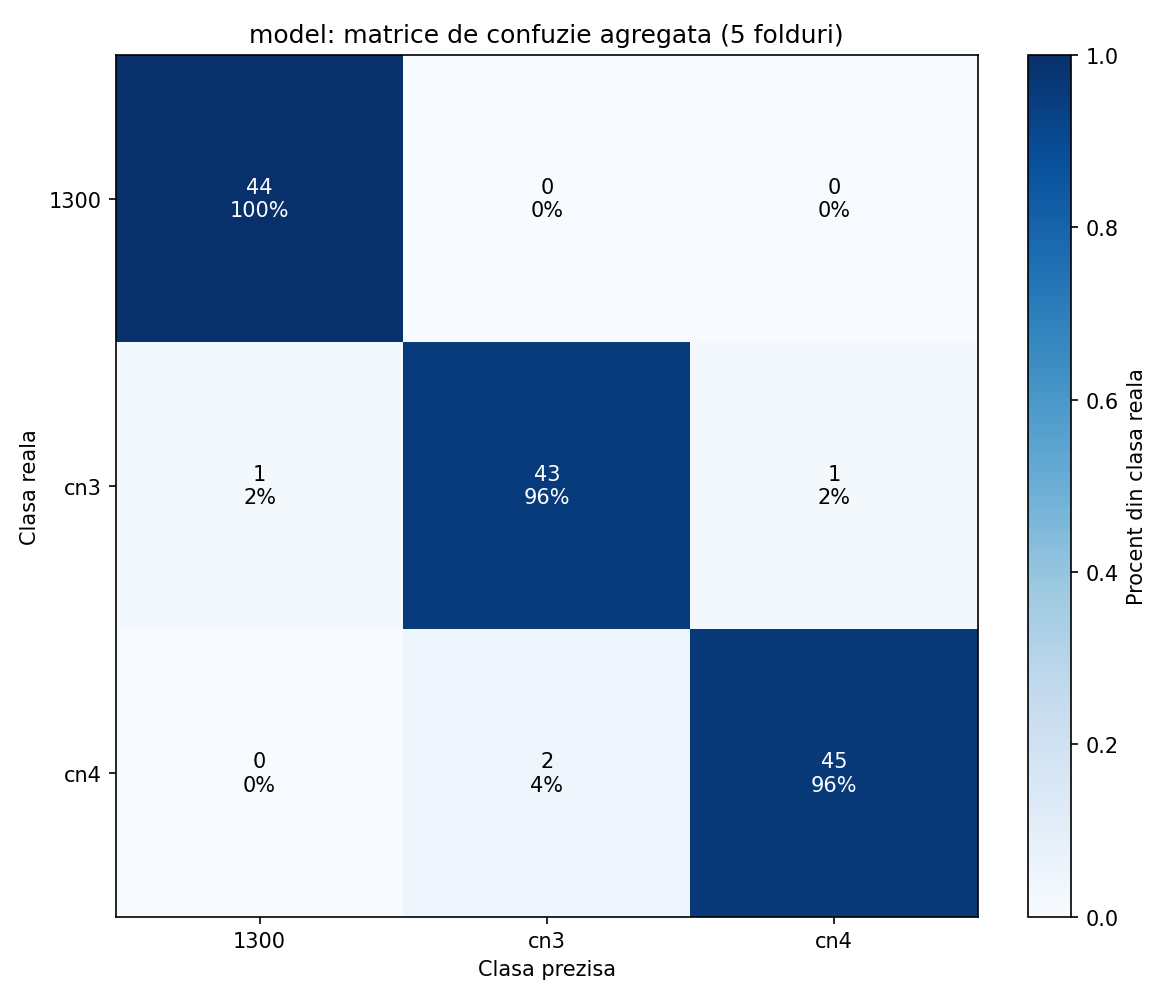
\includegraphics[width=\textwidth]{dinov2_model_confuzie.png}
        \caption{Variantă (1300/CN3/CN4)}
    \end{subfigure}
    \hfill
    \begin{subfigure}{0.48\textwidth}
        \centering
        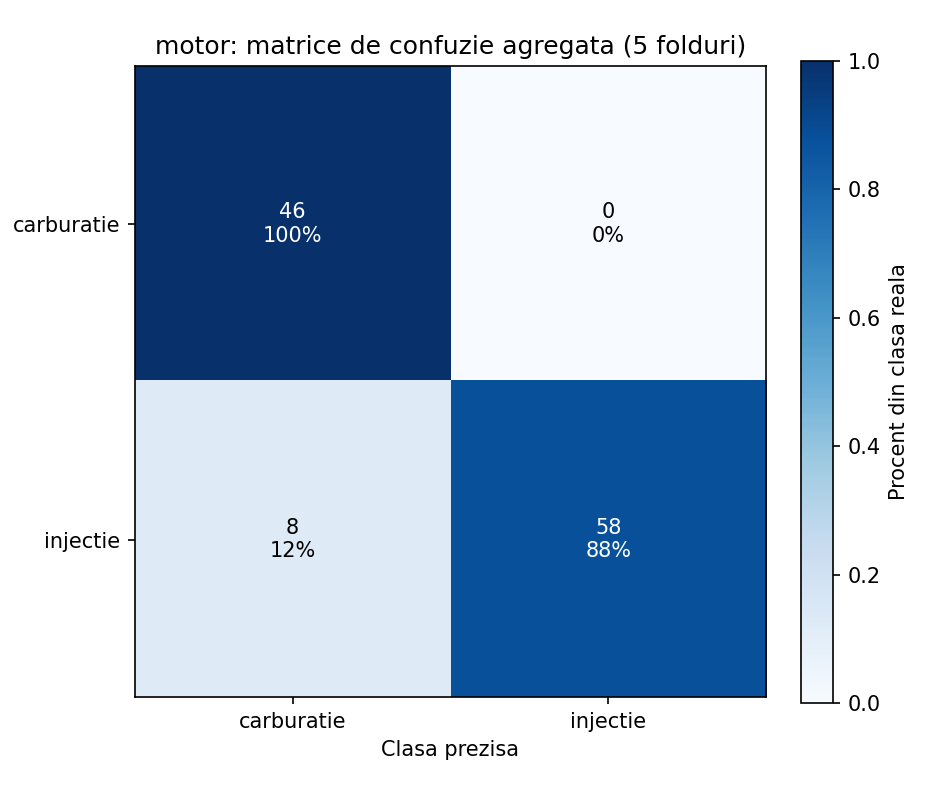
\includegraphics[width=\textwidth]{dinov2_motor_confuzie.png}
        \caption{Motor (carburație/injecție)}
    \end{subfigure}
    \caption{Matricele de confuzie agregate peste cele 5 fold-uri (rând = clasa reală).}
    \label{fig:confuzii}
\end{figure}

\section{Discuție și limitări}

Ierarhia rezultatelor confirmă intuițiile despre dificultatea sarcinilor. Router-ul atinge cea mai bună acuratețe, 98,9\%, deoarece distincția între o vedere frontală, una din spate și compartimentul motor se bazează pe contextul global al imaginii, nu pe detalii fine. Clasificatorul de variantă ajunge la 96,7\%, clasele fiind vizual distincte (faruri rotunde și grilă cromată la 1300, faruri dreptunghiulare la CN3, grilă redesenată la CN4). Caroseria, în schimb, rămâne la 91,6\%: multe vederi din spate sunt fotografiate din unghiuri în care diferența berlină/break se vede greu.

Rezultatul de la motor trebuie citit cu prudență: media de 93,6\% vine cu o deviație standard de 10,5 puncte procentuale, pentru că un fold coboară la 73,1\% în timp ce celelalte patru sunt aproape perfecte. Cu doar 112 imagini de la 97 de vehicule, fiecare fold de validare are în jur de 20 de imagini, deci câteva greșeli schimbă acuratețea cu multe puncte procentuale. Îl considerăm un rezultat preliminar, iar colectarea de date suplimentare pentru această sarcină este principala prioritate.

Mai notăm trei limitări. Prima: metrica are rezoluție mică în general --- la fold-uri de 20--115 imagini, diferențele de 1--2 puncte procentuale între fold-uri sunt zgomot, motiv pentru care raportăm mereu media cu deviația standard, nu o valoare unică. A doua: în setul de variantă, pozele clasei 1300 au rezoluții mai mari (în jur de 850 de pixeli lățime) decât cele din CN3/CN4 (300--500 de pixeli); redimensionarea la $224 \times 224$ atenuează diferența, dar o corelație reziduală între calitatea imaginii și clasă nu poate fi exclusă. A treia: gruparea pe vehicul este semi-automată, deci dacă același autoturism apare în două anunțuri diferite sub identificatori diferiți, o mică scurgere de date poate persista. De asemenea, întreaga evaluare folosește un singur seed; repetarea validării încrucișate cu mai multe seed-uri ar consolida estimările.


\chapter{Concluzii}

Lucrarea a pornit de la o problemă concretă, determinarea automată a configurației tehnice a autoturismelor Dacia 1300/1310, și a condus la un sistem în care un router dirijează imaginea către clasificatorul potrivit, iar predicțiile completează progresiv fișa tehnică. Toate clasificatoarele împart același backbone DINOv2 înghețat, peste care se antrenează câte un strat liniar, iar performanța a fost măsurată prin validare încrucișată grupată pe vehicul, adică pe vehicule nevăzute la antrenare. Rezultatele obținute sunt încurajatoare, principalele limitări ținând de volumul redus și de modul de colectare a datelor.

Sistemul poate fi îmbunătățit din mai multe perspective. În primul rând, extinderea la alte autoturisme, dincolo de gama 1300/1310, ceea ce ar transforma aplicația într-un instrument mai general pentru vehicule de epocă. O a doua direcție este adăugarea unui clasificator pentru culorile de epocă (de exemplu Roșu 28, Portocaliu 331 sau Roșu 25), care ar completa fișa tehnică cu nuanța originală a vehiculului. În final, colectarea de date suplimentare pentru clasificatorul de motorizare, al cărui rezultat este deocamdată instabil între fold-uri, și repetarea validării încrucișate cu mai multe seed-uri ar consolida estimările raportate.

\printbibliography[heading=bibintoc]

% ------- ANEXE -------
\appendix
\titleformat{\chapter}[hang]
  {\normalfont\Huge\bfseries}{\appendixname\ \thechapter}{1em}{}

\chapter{Exemple de imagini din setul de date}
\label{anexa:exemple}

\begin{figure}[H]
    \centering
    \begin{subfigure}{0.35\textwidth}
        \centering
        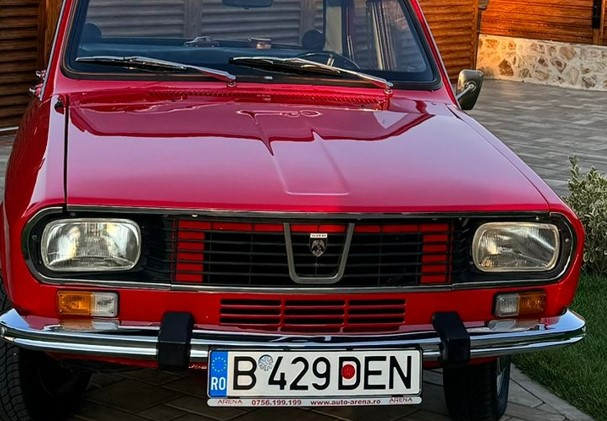
\includegraphics[width=\textwidth]{1300.jpg}
        \caption{Dacia 1300}
    \end{subfigure}
    \hfill

    \vspace{0.5cm}

    \begin{subfigure}{0.35\textwidth}
        \centering
        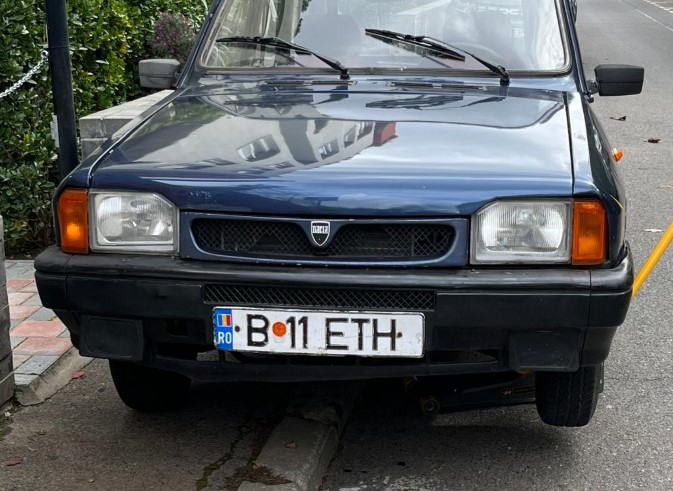
\includegraphics[width=\textwidth]{1310_cn3.jpg}
        \caption{Dacia 1310 CN3}
    \end{subfigure}
    \hfill
    \begin{subfigure}{0.35\textwidth}
        \centering
        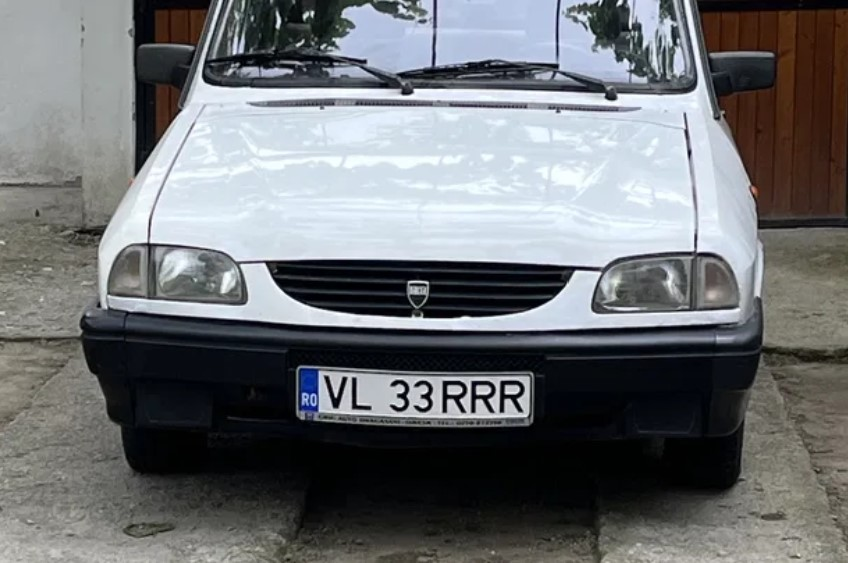
\includegraphics[width=\textwidth]{1310_cn4.jpg}
        \caption{Dacia 1310 CN4}
    \end{subfigure}
    \caption{Exemple de imagini din setul de date, câte una pentru fiecare variantă ce poate fi identificată de clasificatorul pentru modele.}
    \label{fig:exemple_clase}
\end{figure}


\begin{figure}[H]
    \centering
    \begin{subfigure}{0.40\textwidth}
        \centering
        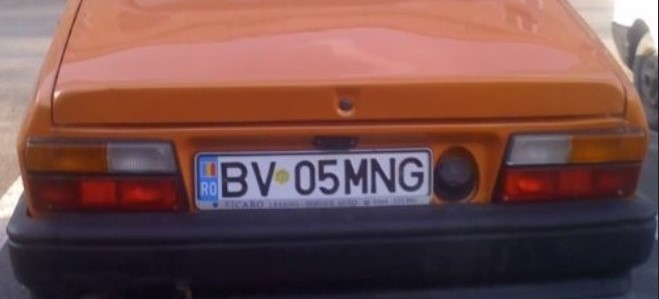
\includegraphics[width=\textwidth]{spate_1310.jpg}
        \caption{Spate Dacia Berlină}
    \end{subfigure}
    \hfill
    \begin{subfigure}{0.40\textwidth}
        \centering
        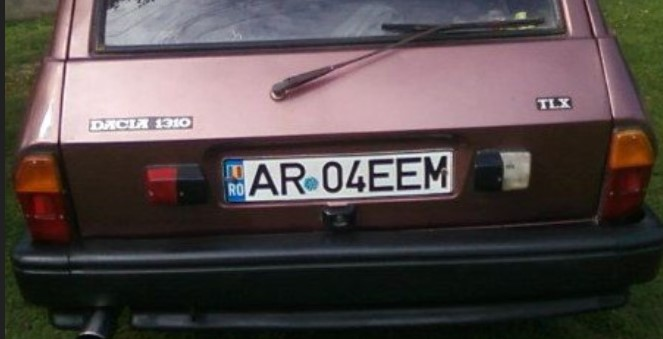
\includegraphics[width=\textwidth]{spate_break.jpg}
        \caption{Spate Dacia break}
    \end{subfigure}
    \caption{Cele două tipuri de caroserie pe care le poate identifica clasificatorul binar pentru șasiuri.}
    \label{fig:exemple_spate}
\end{figure}

\begin{figure}[H]
    \centering
    \begin{subfigure}{0.40\textwidth}
        \centering
        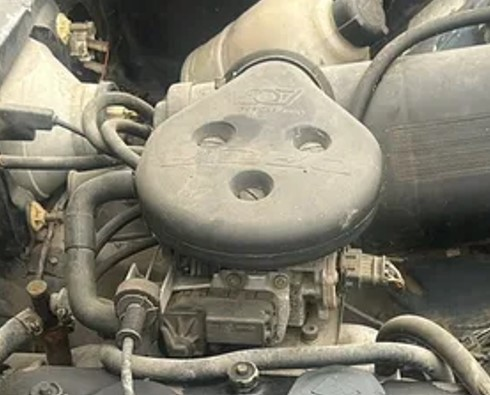
\includegraphics[width=\textwidth]{inj.jpg}
        \caption{Modul de injecție}
    \end{subfigure}
    \hfill
    \begin{subfigure}{0.40\textwidth}
        \centering
        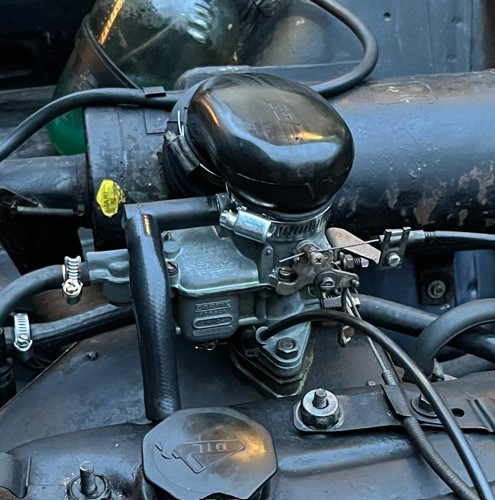
\includegraphics[width=\textwidth]{carbu.jpg}
        \caption{Carburator}
    \end{subfigure}
    \caption{Cele două tipuri de alimentație identificate de clasificatorul pentru motorizări. }
    \label{fig:exemple_motor}
\end{figure}

\chapter{Fragmente de cod}
\label{anexa:cod}

\begin{lstlisting}[caption={Preprocesarea PadToSquare, identică în antrenare și inferență.}, label={lst:padtosquare}]
class PadToSquare:
    def __call__(self, img):
        w, h = img.size
        max_wh = max(w, h)
        padding = ((max_wh - w) // 2, (max_wh - h) // 2,
                   max_wh - w - (max_wh - w) // 2,
                   max_wh - h - (max_wh - h) // 2)
        return F.pad(img, padding, 0, 'constant')
\end{lstlisting}

\begin{lstlisting}[caption={Maparea sursă $\rightarrow$ clasă de router.}, label={lst:mapping}]
MAPPING = {
    "fata":    ["model/1300", "model/cn3", "model/cn4"],
    "spate":   ["caroserie/berlina", "caroserie/break"],
    "motor":   ["motor/carburatie", "motor/injectie"],
}
\end{lstlisting}

\begin{lstlisting}[caption={Logica de respingere.}, label={lst:dispatch}]
top_class, top_prob = scores[0]
if top_prob < REJECT_THRESHOLD:
    print(f"REJECT | top={top_class} ({top_prob*100:.2f}%)")
    return
specialisti = SPECIALIST_MAP.get(top_class, [])
print(f"DISPATCH -> {top_class} | specialisti: {specialisti}")
\end{lstlisting}

\begin{lstlisting}[caption={Antrenarea stratului liniar peste embeddings (full-batch).}, label={lst:probe}]
probe = nn.Linear(384, n_classes)
opt = torch.optim.Adam(probe.parameters(), lr=1e-3,
                       weight_decay=1e-4)
crit = nn.CrossEntropyLoss(weight=class_weights,
                           label_smoothing=0.1)
for epoch in range(200):
    opt.zero_grad()
    loss = crit(probe(X_train), y_train)  # X_train = embeddings
    loss.backward()
    opt.step()
\end{lstlisting}

\chapter{Curbe de antrenare}
\label{anexa:grafice}

\begin{figure}[H]
    \centering
    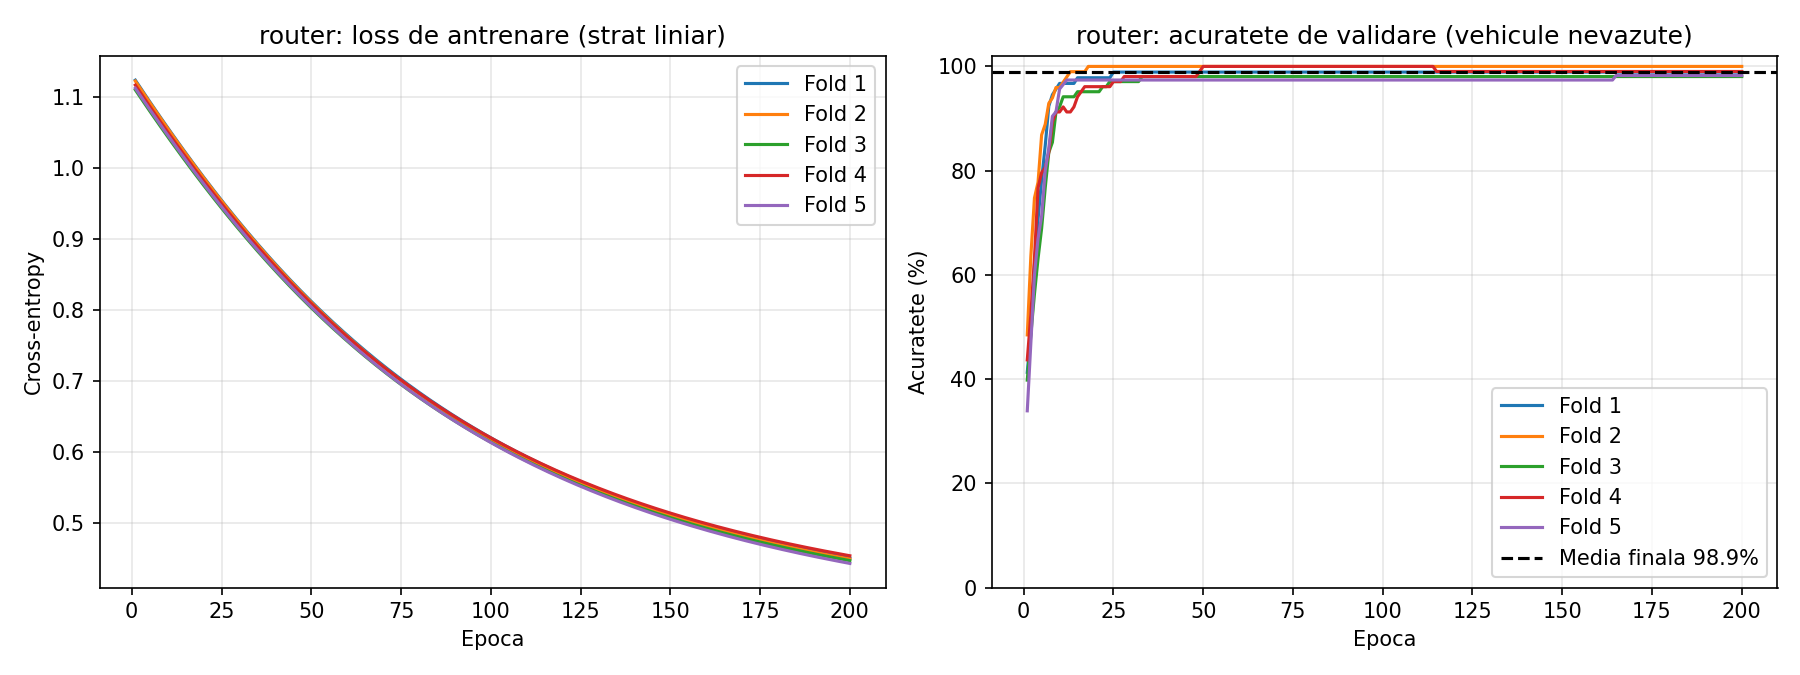
\includegraphics[width=0.95\textwidth]{dinov2_router_training.png}
    \caption{Router-ul (față/motor/spate), 200 de epoci, câte o curbă per fold. Acuratețea de validare se stabilizează rapid, în jurul mediei de 98,9\%.}
    \label{fig:curbe_router}
\end{figure}

\begin{figure}[H]
    \centering
    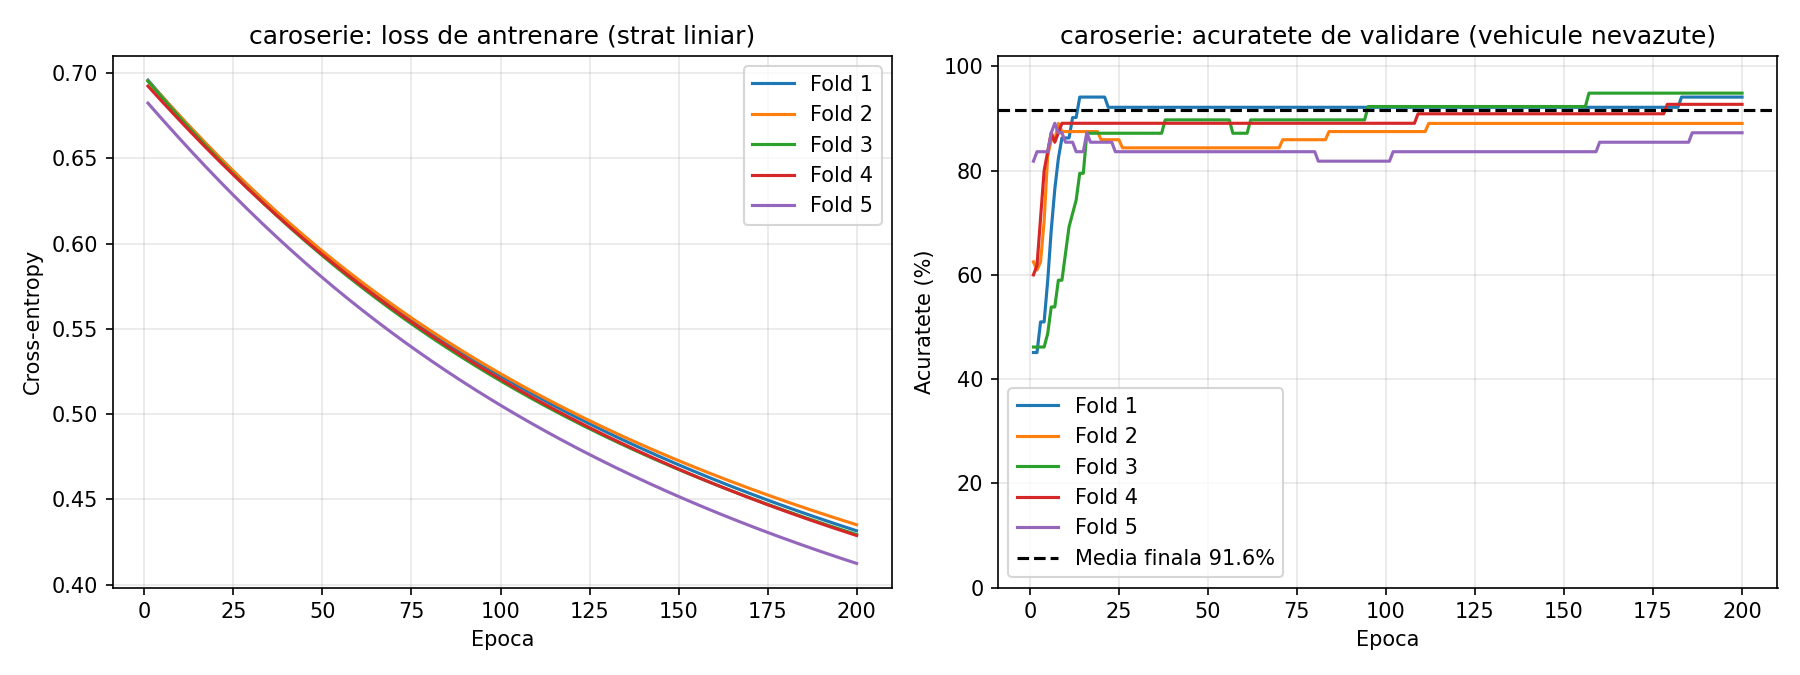
\includegraphics[width=0.95\textwidth]{dinov2_caroserie_training.png}
    \caption{Clasificatorul de caroserie (berlină/break). Acuratețea de validare se stabilizează în jurul valorii de 91--92\%, cu diferențe vizibile între fold-uri.}
    \label{fig:curbe_caroserie}
\end{figure}

\chapter{Reguli și paginile aplicației}
\label{anexa:reguli}

Pe lângă atributele prezise direct de clasificatori, aplicația completează fișa
tehnică și cu valori derivate determinist din varianta detectată, conform
regulilor din Tabela~\ref{tab:derivare}.

\begin{table}[H]
\centering
\caption{Reguli folosite de aplicație.}
\label{tab:derivare}
\renewcommand{\arraystretch}{1.3}
\begin{tabular}{>{\raggedright\arraybackslash}p{3.3cm}
                >{\raggedright\arraybackslash}p{2.2cm}
                >{\raggedright\arraybackslash}p{4.2cm}
                >{\raggedright\arraybackslash}p{3.6cm}}
\toprule
\textbf{Varianta detectată} & \textbf{Capacitate cilindrică} &
\textbf{Alimentare} & \textbf{Aprindere} \\
\midrule
Dacia 1300 & 1289 cm\textsuperscript{3} &
Carfil 32 IRM / Solex 32 EISA-3 & Distribuitor Ducellier 4224 \\
\addlinespace
Dacia 1310 CN3 & 1289/1397 cm\textsuperscript{3} &
Carfil 32 IRM & Distribuitor I.E.P.S 3239 \\
\addlinespace
Dacia 1310 CN4 & 1397 cm\textsuperscript{3} &
Injecție monopunct Bosch & Electronică, comandată de ECU \\
\bottomrule
\end{tabular}
\end{table}
\newpage

\begin{figure}[H]
    \centering
    \begin{subfigure}{0.9\textwidth}
        \centering
        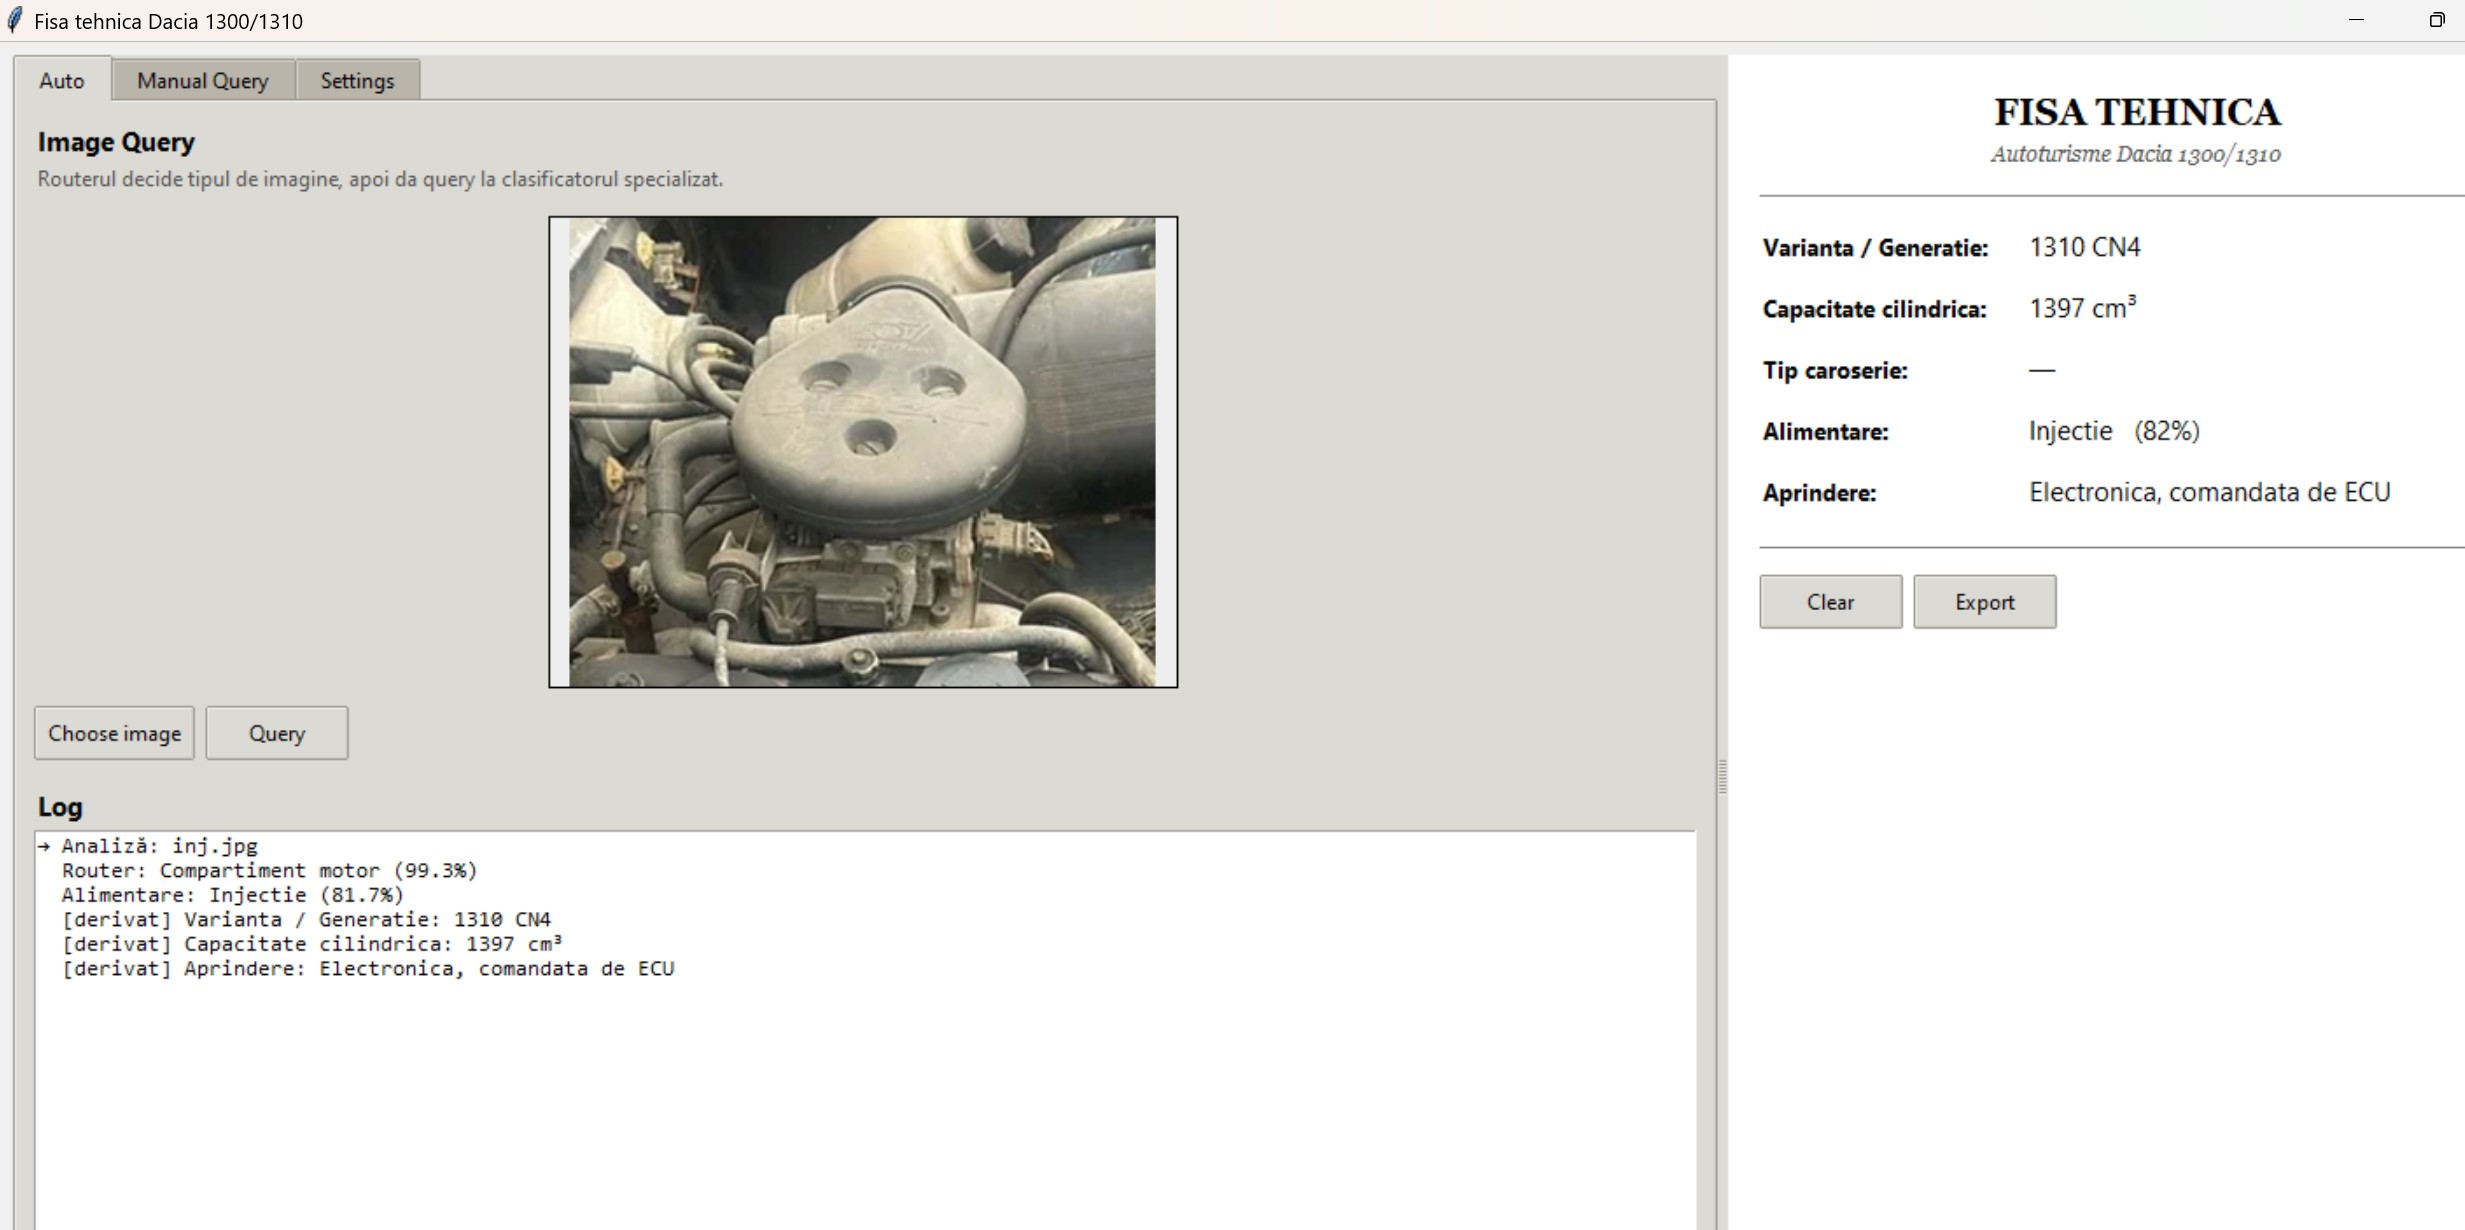
\includegraphics[width=\textwidth]{captura1.jpg}
        \caption{Modul \textbf{Auto}: routerul decide tipul imaginii și completează fișa.}
        \label{fig:captura1}
    \end{subfigure}
    \vspace{0.6cm}
    \begin{subfigure}{0.9\textwidth}
        \centering
        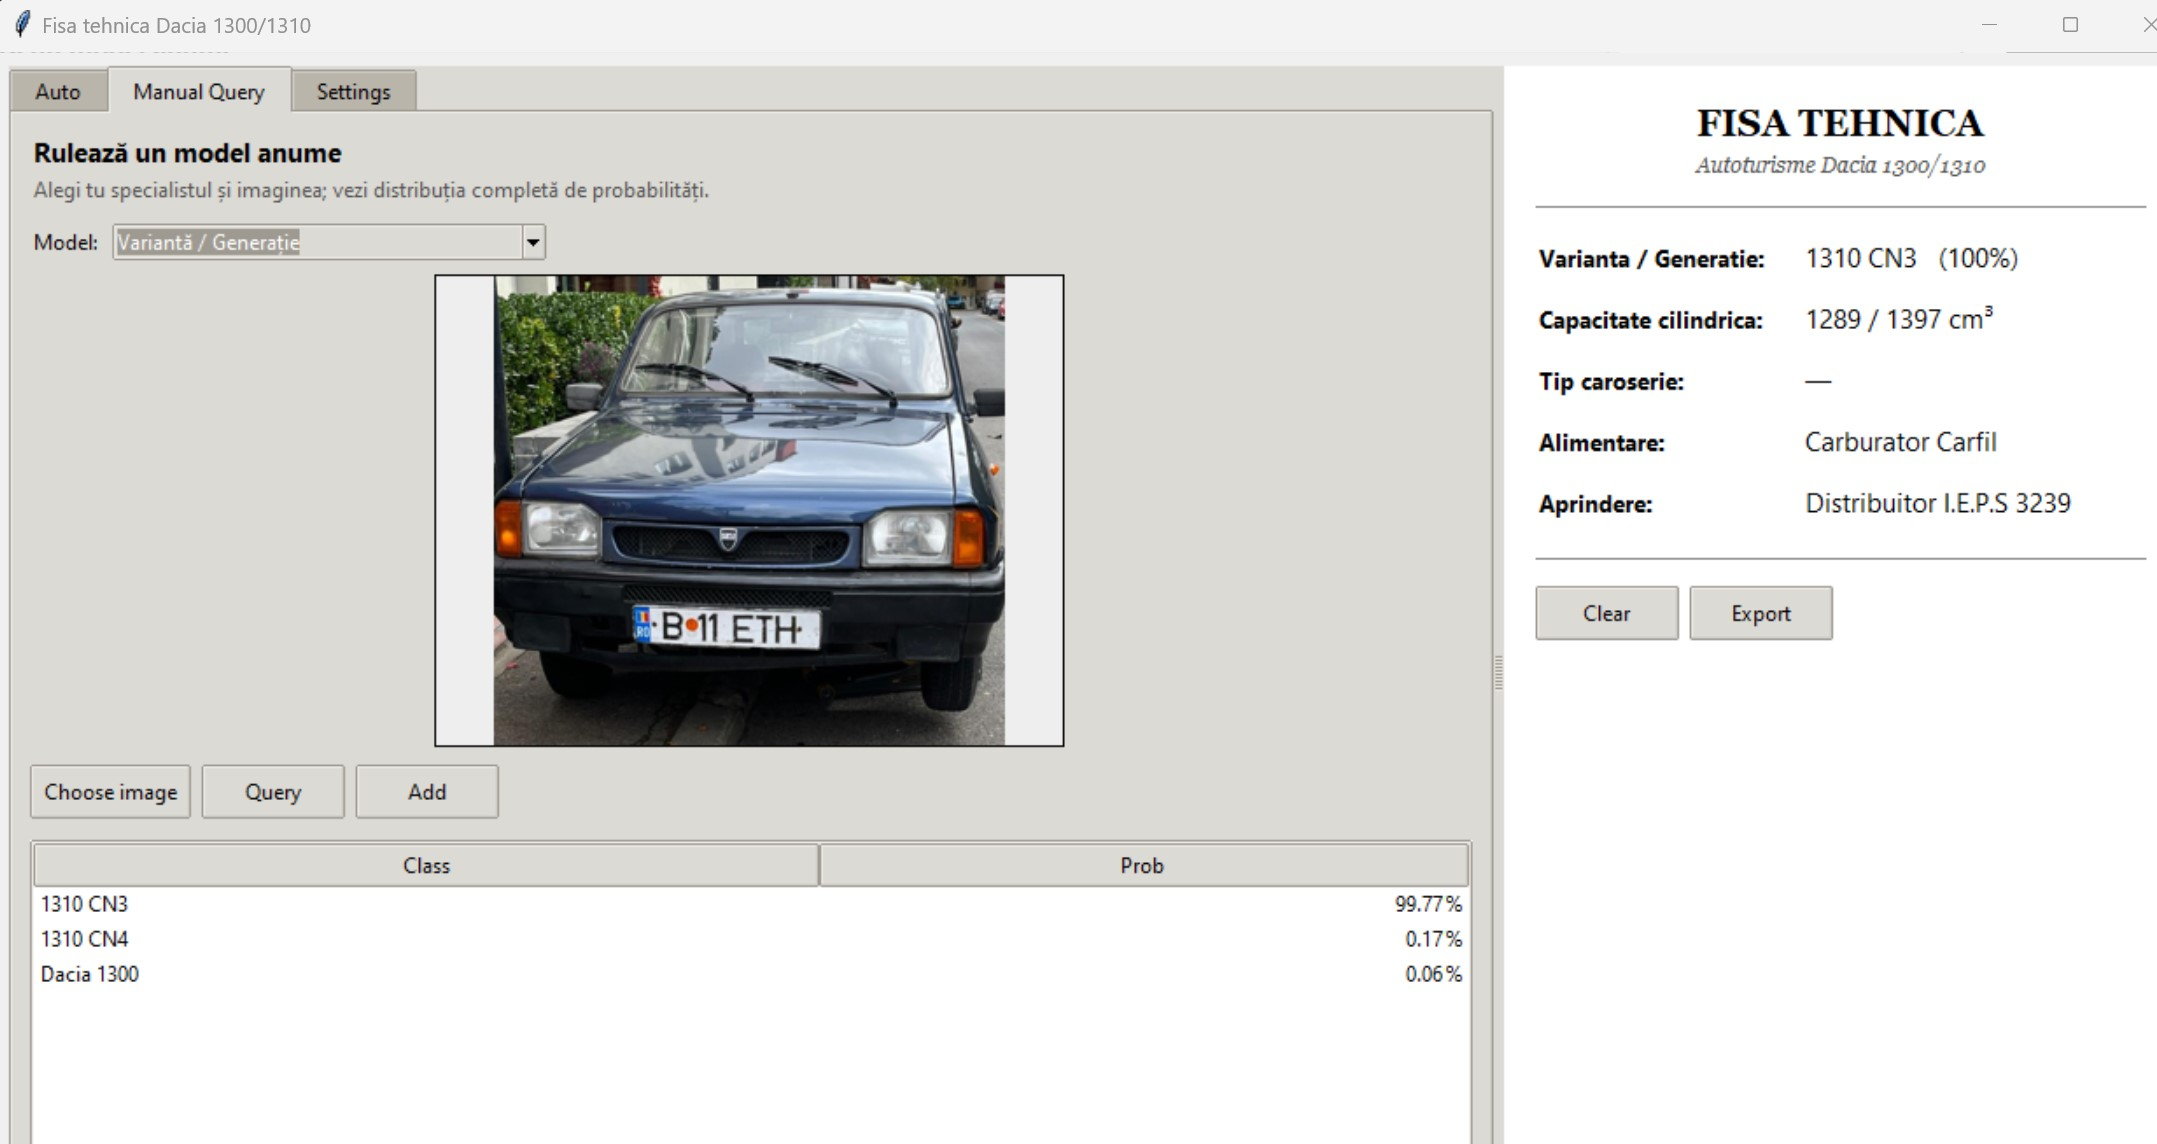
\includegraphics[width=\textwidth]{captura2.jpg}
        \caption{Modul \textbf{Manual}: distribuția de probabilități pe clase.}
        \label{fig:captura2}
    \end{subfigure}
    \caption{Capturi de ecran din aplicație.}
    \label{fig:capturi}
\end{figure}

\clearpage

\begin{figure}[H]
    \centering
    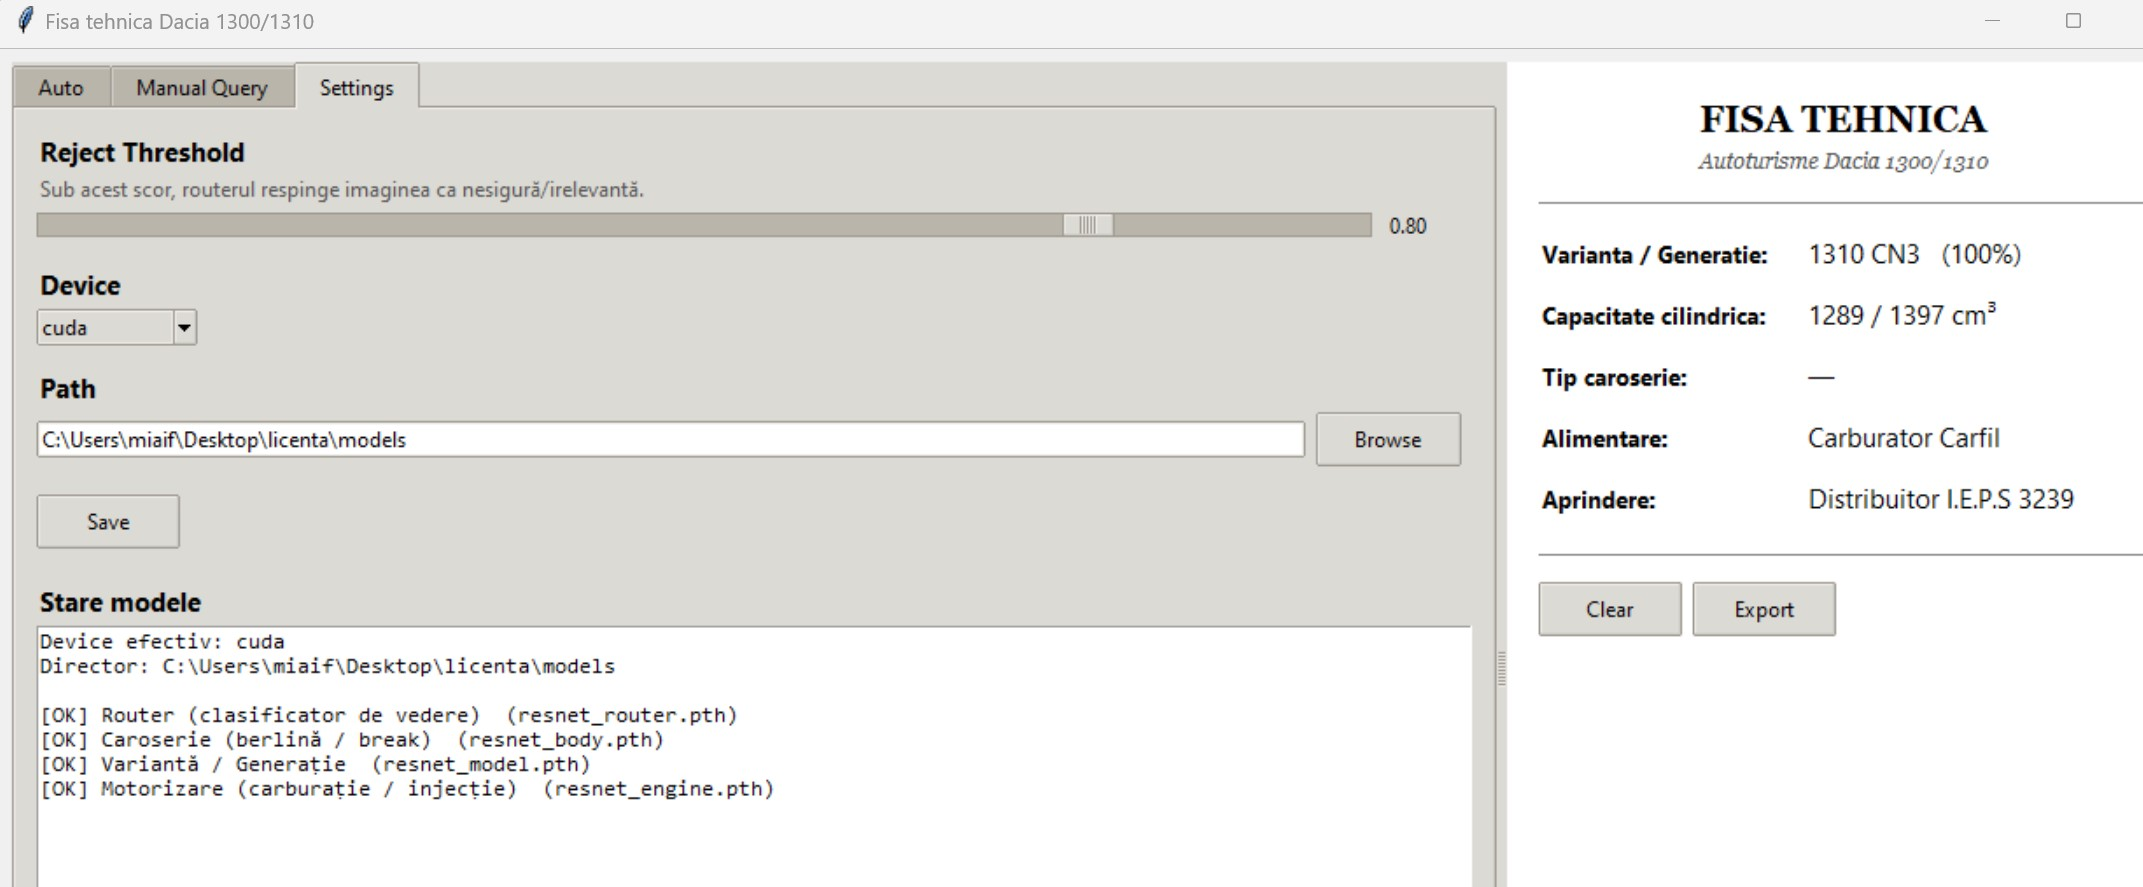
\includegraphics[width=0.9\textwidth]{captura3.jpg}
    \caption{Tab-ul \textbf{Settings}: configurarea pragului și a căilor.}
    \label{fig:captura3}
\end{figure}

\end{document}
